\chapter{Objektorientierter Entwurf}


\section{Lernziele}

\begin{itemize}
    \item für kleinere Projekte qualitätssichernde Maßnahmen planen und verfolgen können
    \item Tests planen und dokumentieren können
    \item gefundene Fehler geeignet verwalten können
\end{itemize}

\section{Von der Analyse zum Entwurf}

\noindent
Im \textbf{Entwurf} beschreiben Entwickler


\begin{itemize}
    \item aus welchen \textbf{Klassen}, \textbf{Methoden} oder \textbf{Dateien} das zu entwerfende System bestehen soll
    \item wie diese Bauteile aussehen sollen
    \item in welcher Beziehung sie zueinander stehen sollen
    \item wie diese Bauteile zusammenarbeiten
\end{itemize}

\noindent
Im \textbf{objektorientierten Entwurf} bedeutet dies

\begin{itemize}
    \item das Erstellen von Klassen samt deren Attribute und Methode
    \item das Festlegen der Assoziationen und Vererbungsbeziehungen
    \item das Beschreiben des Zusammenspiels der Instanzen
\end{itemize}

\subsection*{Basis, Anforderungen, Analyse und Architektur}
Der Entwurf geschieht auf Grundlage der Anforderungen und der Ergebnisse der Analyse und innerhalb der gewählten Architektur.\\

\noindent
Aus den Anforderungen sind für den Entwurf die \textbf{funktionalen Anforderungen} wichtig.\\
Die \textbf{nicht-funktionalen Anforderungen} sind bereits in der Architektur berücksichtigt.\\

\noindent
Die Architektur liefert die Bauteile für die Software, der Entwurf konkretisiert diese dann anhand der funktionalen Anforderungen.\\

\noindent
Die Ergebnisse der \textbf{Analyse} in Form des \textbf{Domänenmodells} ist Grundlage für die \textit{Datenhaltung} in der Anwendung und für eventuelle \textit{Datenbankschemas}.\\

\noindent
Die \textbf{Definition} der Schnittstellen, insb. der GUI, bilden die Basis für den Entwurf der technischen Umsetzung der Schnittstelle.

\subsection*{Vor- und Nachteile}
Probleme werden meist erst beim Modellieren klar.
Es bietet sich deshalb an, erst einen groben Entwurf zu skizzieren.
Der Entwurf kann (eindeutige) Absprachen unter den Projektbeteiligten erleichtern.\\

\noindent
Größere Entwürfe bzw. sehr detaillierte sollten im ersten Anlauf vermieden werden - stattdessen sollte iterativ gearbeitet werden: Es werden erst Teile entworfen und umgesetzt, und basierend auf den gemachten Erfahrungen werden Entwürfe angepaßt.



\section{Klassen im Entwurf}

Im Unterschied zu den Entwürfen aus der Analyse  beschreiben Klassen des Entwurfs nicht fachliche Zusammenhänge, sondern Klassen, die in der gewählten objektorientierten Sprache umgesetzt werden.\\

\noindent
Damit besitzen die Klassen des Entwurfs \textbf{technische Verantwortichkeiten}, wie

\begin{itemize}
    \item Datenhaltung (\textit{Entity})
    \item Durchführung von Berechnungen
    \item Überprüfung von Regeln
    \item Interaktion mit dem Anwender (\textit{User Interface})
    \item Ablaufsteuerung (\textit{Control})
    \item Schnittstellen zu anderen Systemen (\textit{Boundary})
    \item Services für andere Klassen (\textit{Utility})
\end{itemize}

\subsection*{Eine Verantwortlichkeit pro Klasse}
Wie in der Analyse gilt: jede klasse sollte eine, max. zwei Verantwortlichkeiten besitzen.\\
$\rightarrow$ die Klassen werden dadurch leichter verständlich und änderbar.\\

\noindent
Klassen mit ähnlichen Verantwortlichkeiten werden gemeinsam in \textbf{Schichten} oder \textbf{Module}\footnote{
bspw. \textit{Pakete} bei \textit{Wedemann} (vgl.\cite[49]{Wed09b}). In einem System mit hoher \textit{Kohäsion} liegt eine starke funktionale Abgrenzung der Module, Klassen und Methoden vor (vgl.\cite[310 ff.]{Dem79}).
} verteilt.\\
Viele Klassen, die jeweils wenig Funktionalität besitzen, sind einfacher zu verstehen, als wenig Klassen, die unübersichtlich viel Funktionalität besitzen (vgl. \cite[49]{Wed09b})}\footnote{
s. a. \textit{Martin} in \cite[95, The Single-Responsibility Principle]{Mar03}: ``A class should have only one reason to change ``
}. \\



\noindent
Die \textbf{Übersicht} über die Vielzahl der Klassen wird durch einen \textbf{sauberen Entwurf} gewährleistet.
\section{Strukturen und Verhalten}
Wie bei der Analyse bestehen auch Klassen des Entwurfs aus \textbf{statischen} und \textbf{dynamischen Modellen}.\\

\noindent
Statische Modelle werden durch \textbf{Paket-} und \textbf{Klassendiagramme} beschrieben\footnote{
\textit{Paketdiagramme} werden auch zur Dokumentation der Architektur genutzt.
}.\\

\noindent
Dynamische Modelle werden durch \textbf{Zustands-} und \textbf{Sequenzdiagramme} beschrieben\footnote{
\textit{Wedemann} weist darauf hin, dass auch \textit{Aktivitätsdiagramme} eingesetzt werden, allerdings \textit{Sequenzdiagramme} im Entwurf von Praktikern für sinnvoller erachtet werden (vgl.\cite[49]{Wed09b}).
}.\\

\noindent
\textbf{Klassendiagramme} werden wie in der Analyse eingesetzt, allerdings kommen im Entwurf technische Details dazu, wie die \textit{Sichtbarkeiten}, die \textit{Typen} von Attributen, Rückgabewerten und formalen Parametern.\\
Es empfiehlt sich, Gerüstmethoden wie \textit{Getter}/\textit{Setter} sowie Konstruktoren der Übersicht halber wegzulassen (s. \cite[50]{Wed09b}).\\

\noindent
\textbf{Sequenzdiagramme} modellieren den zeitlichen Ablauf von Nachrichten zwischen Objekten.\\
Für Notation und Beispiele s. Abschnitt~\ref{sec:sequenzdiagramme}.
\section{Vorgehen beim Entwerfen}
Die Art und Weise, wie Klassen und ihr Zusammenspiel modelliert werden, hängt von der Aufgabenstellunf und der gewählten Architektur ab.\\

\noindent
Typischerweise wird mit dem Entwurf der Datenhaltung begonnen.\\
Hierzu werden die Klassen des \textbf{Domänenmodells} als Grundlage genutzt.\\

\noindent
Nacheinander werden Klassen entworfen, die, für die \textbf{Erfüllung der funktionalen Anforderungen} verantwortlich sind, und anschließend in Quelltext umgesetzt.\\

\noindent
Zunächst werdn die Klassen und ihre Beziehungen in einem Klassenmodell entworfen.\\

\noindent
\textbf{Sequenzdiagramme} werden meist nur für ausgewählte Abläufe modelliert, um zu prüfen, ob die entworfenen Klassen für die Abläufe geeignet sind, und zum anderen für die Dokumentation schwieriger oder unklarer Abläufe.\\

\noindent
Für den Entwurf werden \textbf{Entwurfsmuster} genutzt.\\

\noindent
Beachtet werden sollte insgesamt, dass nicht alles auf einmal modelliert wird (``Model in small increments``\footnote{\cite[51]{Wed09b}}), da meistens nicht alles von Beginn an richtig entworfen werden kann.
Entwürfe werden durch die Implementierung im Quelltext erst erprobt (``Prove it with code``\footnote{
    s.a. Abschnitt~\ref{sec:softwarearchitektur}
}).

\subsection*{Bewährte Prinzipien}

Die folgenden Prinzipien gehen zurück auf \textit{Ambler}, \cite[112, Table 4.2. The Supplementary Principles of AM]{Amb04}:

\begin{itemize}
    \item \textbf{Travel light}: Anforderungen ändern sich im Laufe eines Projektes.
    Diagramme sollten deshalb kritisch überprüft werden, ob sie Wert für die weitere Entwicklung haben, oder ob sie unter Verzicht auf weitere Aktualisierung archiviert order verworfen werden
    \item \textbf{Detailtiefe nach Problemstellung}: Es ist nicht immer sinvoll, Entwürfe formal detailliert auszugestalten, da manche Dinge für das verständnis nicht wichtig sind, wie bspw. \textit{Setter}/\textit{Getter} oder Sichtbarkeiten in einem Klassendiagramm.
    \item \textbf{Iterate to another artifact}: Stagniert die Arbeit an einem Diagramm, kann es eine gute Idee sei, mit einem anderen Diagrammtyp weiterzumachen: Geht es in einem Klassendiagramm nicht weiter, kann ggf. ein Objektdiagramm oder die Darstellung dynamischen Verhaltens anhand eines Sequenzdiagrammes das Verständnis fördern.
    \item \textbf{Model with others}: ``Software development is a lot like swimming: it is very dangerous to do it alone; it is also best to swim with people who know how to swim (they should at least know how to stay afloat).`` (\cite[52]{Amb04}\footnote{
    \textit{Wedemann}: Modellieren ist im Team effektiver und macht mehr Spaß (vgl.~\cite[52]{Wed09b})
    })
\end{itemize}

\section{Entwurfsmuster}

\textbf{Entwurfsmuster} (\textit{Design Patterns}) sind wie Analyse- (s. Abschnitt~\ref{sec:analysemuster}) und Architekturmuster (s. Abschnitt~\ref{sec:architekturmuster}) vorgefertigte Lösungsschablonen für verallgemeinerte Probleme des Entwurfs.\\

\noindent
Entwurfsmuster müssen zur Lösung konkreter Aufgaben angepasst werden.

\subsection{Beobachter (Observer)}

\subsubsection*{Problem}
\begin{itemize}
    \item eine Klasse soll die Möglichkeit haben, anderen Klassen Nachrichten zu senden
    \item der Typ der empfangenden Klasse soll vorher nicht bekannt sein
\end{itemize}

\subsubsection*{Lösung}
\begin{itemize}
    \item eine Klasse, die vom Typ \code{Observable} ist, besitzt Referenzen auf Objekte, die \code{Observer} (\textit{Nachrichtenempfänger})implementieren
    \item Beobachter registrieren sich bei den zu beobachtenden Objekten
    \item Nachrichten werden ausgehend von \code{Observable} (bspw. über \code{notify()}) an die \code{Observer} geschickt
\end{itemize}

Das Entwurfsmuster ist auch unter \textit{publish-subscribe} bekannt.


\begin{figure}
    \centering
    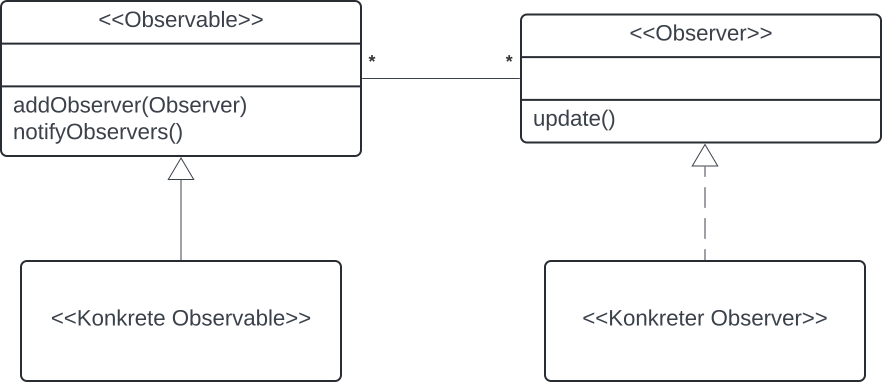
\includegraphics[scale=0.4]{part two/Objektorientierter Entwurf/img/observer}
    \caption{Klassendiagramm des Observer-Patterns (Quelle: eigene)}
    \label{fig:observer}
\end{figure}

\subsection{MVC (Model-View-Controller)}

\subsubsection*{Problem}

\begin{itemize}
    \item eine Anwendung verarbeitet Eingaben und reagiert (interaktiv) mit Ausgaben
    \item die Ausgaben sollen über eine Aktualisierung des GUI erfolgen
    \item es stellt sich die Frage, wie die Verantwortlichkeiten sinnvoll verteilt werden können
\end{itemize}

\subsubsection*{Lösung}
Die Verantwortlichkeiten werden unterteilt in

\begin{itemize}
    \item \textbf{Model}: beinhalten Daten und fachliche Funktionalitäten
    \item \textbf{View}: zeigen Daten (des Models) an
    \item \textbf{Controller}: nehmen Eingabedaten entgegen, speichern Daten im Model und steuern Elemente des UI
\end{itemize}

\noindent
Hierbei reagiert die \textbf{View} auf Änderungen im \textbf{Model}, die View ist also ein \textbf{Beobachter} des Models (\textbf{Observable}).\\
Der \textbf{Controller} verarbeitet Nutzerinteraktionen und kommuniziert diese an das Model.\\
In der Hinsicht ist der Controller ein Observer für die GUI-Elemente, die Nutzerinteraktionen verarbeiten (s. Abbildung~\ref{fig:mvc}).

\begin{figure}
    \centering
    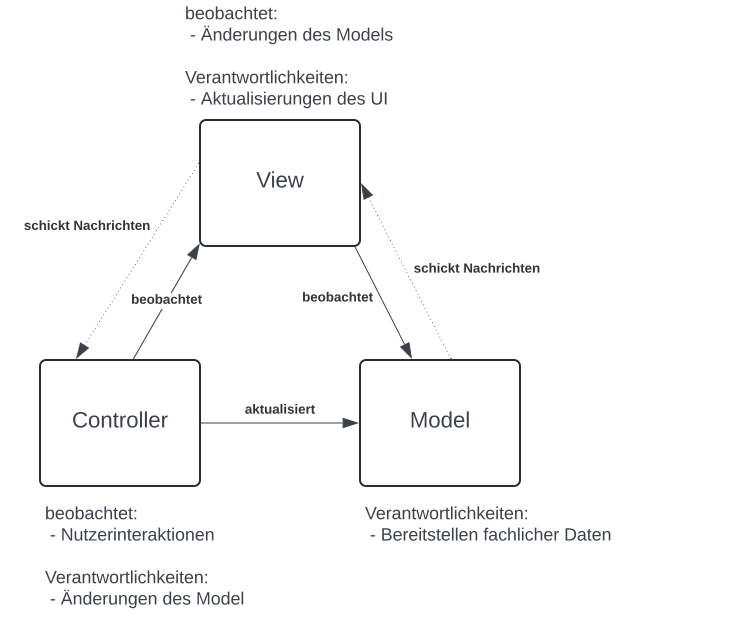
\includegraphics[scale=0.4]{part two/Objektorientierter Entwurf/img/mvc}
    \caption{Schematische Darstellung des MVC-Patterns mit seinen Verantwortlichkeiten (Quelle: eigene)}
    \label{fig:mvc}
\end{figure}

\subsubsection*{Vorteile}
Die Vorteile sind eine klare Trennung der Verantwortlichkeiten sowie die hierdurch bedingte lose Kopplung der Komponenten untereinander, was ein Testen sowie Austauschen der eingesetzten Komponenten vereinfacht.

\subsection{Immutable}\label{subsec:immutable}

\subsubsection*{Problem}
\begin{itemize}
    \item Referenzen auf Instanzen werden von einem Objekt an andere Objekte weitergegeben
    \item Änderungen der Inhalte der Referenzen wirken sich unerwünscht auf andere Objekte aus\footnote{
    auch bekannt als \textbf{Aliasing Bug}, s. \url{https://martinfowler.com/bliki/AliasingBug.html}, abgerufen 17.04.2024
    }
\end{itemize}

\subsubsection*{Beispiel}

\begin{minted}[mathescape,
    linenos,
    numbersep=5pt,
    gobble=2,
    fontsize=\small,
    frame=lines,
    framesep=2mm]{java}

    class Date {
        public Date(String d) {
            day = d;
        }
        public void setDay(String d) {
            day = d;
        }
    }

    class CalendarEvent {
        Date when;
        public CalendarEvent(Date w) {
            when = w;
        }
        public Date when() {
            return when;
        }
    }

    Date when = "Monday";
    CalendarEvent concertEvent = new CalendarEvent(when);
    CalendarEvent readingEvent = new CalendarEvent(when);

    // ändert gleichzeitig den Veranstaltungstag
    // von readingEvent
    concertEvent.getWhen().setDay("Tuesday");

\end{minted}


\subsubsection*{Lösung}

\begin{itemize}
    \item Attribute im Konstruktor definieren
    \item nur \code{get*}-Methoden implementieren, aber keine \code{set*}-Methoden
    \item es wird keine Methode implementiert, die den \textbf{internen Zustand} des Objektes verändert
    \item sollte eine Änderung des internen Zustands benötigt sein, wird eine neue Instanz der Klasse mit den
    gewünschten Aktualisierungen erzeugt - das ursprüngliche Objekt bleibt so unverändert\footnote{
        Anwendung bspw. in \textbf{Value Object}s, vgl.~\cite[486]{Fow03}
    }
    \item die entsprechende Klasse sollte als \code{final} deklariert werden, damit es nicht möglich ist, abgeleitete Klassen zu erzeugen, in denen das Verhalten geändert wird
\end{itemize}

\subsubsection*{Probleme und Alternativen}
Sollten trotzdem die Eigenschaften eines Objektes oft geändert werden müssen, sollten die Klassen als \textit{mutable} implementiert werden, aber die \textit{Getter} der privaten Objekte sollten dann \textbf{Kopien} dieser Objekte zurückliefern.

\subsection{Iterator}

\subsubsection*{Problem}
\begin{itemize}
    \item Objekte sind in verschiedenen Datenstrukturen wie \textit{verkettete Liste}, \textit{Baum} oder \textit{Vektor} (sog. \textbf{Aggregaten}) organisiert
    \item sollen Methoden sequentiell auf alle Objekte zugreifen, die ein Aggregat beinhalten, muss für jede Datenstruktur der Zugriff anders organisiert werden\footnote{
    Baum wird in bestimmter Reihenfolge traversiert, auf ein Array wird über einen Laufindex zugegriffen usw.
    }
    \item die Struktur soll verborgen bleiben, damit sie für den sequentiellen Zugriff unerheblich ist; die Datenstruktur wird darüber leicht austauschbar
\end{itemize}

\subsubsection*{Lösung}
Es wird von dem verwendeten Framework / der Programmiersprache ein \textbf{Iterator} zur Verfügung gestellt (s. Abbildung~\ref{fig:iterator}).


\begin{figure}
    \centering
    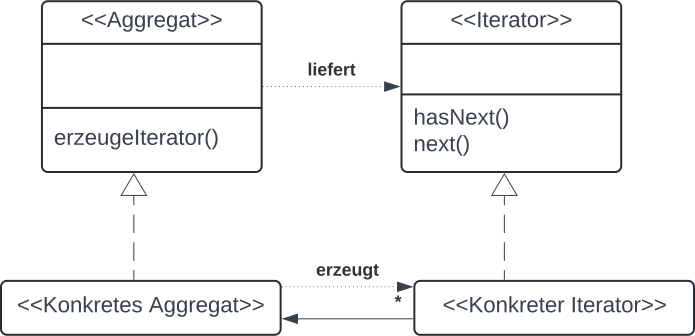
\includegraphics[scale=0.4]{part two/Objektorientierter Entwurf/img/iterator}
    \caption{Klassendiagramm des Iterator-Patterns (Quelle: in Anlehnung an~\cite[60, Abb. 3.9]{Wed09b})}
    \label{fig:iterator}
\end{figure}


\subsection{Fassade}

\subsubsection*{Problem}
\begin{itemize}
    \item Klassen nutzen eine zusammengehörige Gruppe von zusammenarbeitenden Klassen
    \item die Details der Gruppe sollen verborgen bleiben, damit einzelne Bestandteile leichter geändert oder ausgetauscht werden können
\end{itemize}

\subsubsection*{Lösung}
\begin{itemize}
    \item Bereitstellen einer Klasse, die eine \textbf{Fassade} repräsentiert
    \item die Klasse stellt Methoden bereit, die eine Untermenge der Funktionalität des Systems bereitstellt
    \item andere Klassen kennen die öffentliche Schnittstelle der Fassade und greifen nur noch auf diese zu
    \item die Fassade delegiert die Aufrufe an die Objekte, aus denen die Fassade besteht
\end{itemize}

\subsubsection*{Vorteile}
Die Fassade stellt die \textbf{Abstraktion der Gruppe} dar (vgl. \cite[61]{Wed09b}, s. Abbildung~\ref{fig:fassade}).

\begin{itemize}
    \item Benutzung der Gruppe von Klassen wird über einheitliche Schnittstelle vereinfacht
    \item Veränderungen hinter der Fassade bleiben ohne Auswirkungen auf die Nutzer der Fassade
    \item es ist nur die Schnittstelle der Fassade zu verstehen, nicht die Details der Gruppe
\end{itemize}

\begin{figure}
    \centering
    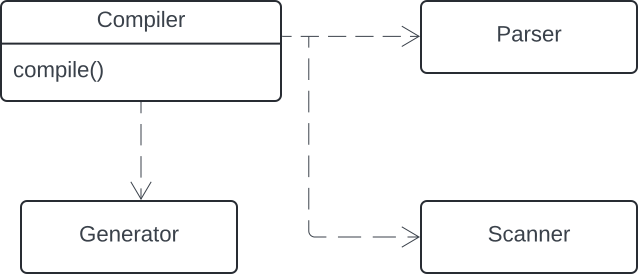
\includegraphics[scale=0.4]{part two/Objektorientierter Entwurf/img/fassade}
    \caption{Informelle Darstellung der Arbeitsweise einer Fassdade (Quelle: eigene)}
    \label{fig:fassade}
\end{figure}

\section{Beispiel eines Entwurfs}
\textit{Wedemann} gibt in~\cite[63 ff.]{Wed09b} ein Beispiel für einen Entwurf, indem er wie folgt vorgeht:

\begin{enumerate}
    \item Aufteilung der User Story in Anwendungsfälle
    \item \textbf{Analyseergebnis}:
    \begin{itemize}
        \item  Aus den funktionalen Anforderungen extrahiert er das \textbf{Domänenmodell}, das in ein (wenig detailliertes) UML-Klassendiagramm überführt wird
        \item  ein \textbf{fachlicher Dialogentwurf} zeigt eine grobe Skizze des UI mit einigen Interaktionselementen
    \end{itemize}
    \item \textbf{Entwurf}:
    \begin{itemize}
        \item ein \textbf{technischer Dialogentwurf} erweitert den fachlichen Dialogentwurf um konkrete Typen der einzelnen Interaktionselemente und verwendeten Komponenten
        \item das Klassendiagramm der Analyse wird erweitert, Klassendiagramme der Komponenten werden hinzugefügt und um technischen Details ergänzt
    \end{itemize}
\end{enumerate}

\noindent
\textit{Wedemann} weist darauf hin, dass bei dem Entwurf darauf geachtet werden sollte, dass die Verantwortlichkeiten so verteilt werden sollen, dass die einzelnen Klassen eine bis max. zwei Verantwortlichkeiten übernehmen.\\

\noindent
Sollten außerdem Erfahrung mit Entwurfsmustern und (eingesetzten) Programmiersprachen und Frameworks fehlen, empfiehlt es sich, zunächst kleinteilig zu entwerfen und im Anschluss zu implementieren (\textit{Prove it with code}, \textit{Model in small increments}).
Er weist aber darauf hin, dass dieses Vorgehen den Nachteil hat, dass Probleme in späteren Teilen entstehen können, wenn bestimmte Funktionalität (oder auch Muster) nicht erkannt wurde und diese nachträglich eingefügt werden muß.\\
Er empfiehlt, Prototypen zu bauen\footnote{
    \textit{Throw-Aways} - also Prototypen, die verworfen werden
}.\\
\textit{Thomas und Hunt} wissen über diesen Prozess:

\blockquote[{\cite[57]{TH19}}]{
Prototyping is a learning experience. Its values lies not in the code produced, but in the lessons learned. That's really the point of prototyping.
}

\noindent
Demgemäß sollen die daraus gewonnenen Erkenntnisse und Erfahrungen im Anschluss zur Erstellung des Systems genutzt werden.

\section{Prinzipien guten Entwurfs}

Der Abschnitt~\cite[69, 3.7 Prinzipien guten Entwurfs]{Wed09b} vermittelt Kenntnisse, anhand derer man

\begin{itemize}
    \item Kriterien kennt, anhand derer man gute und weniger gute Entwürfe unterscheiden kann
    \item die Güte eines Entwurfs beurteilen kann
    \item besserer Entwürfe erstellen kann
\end{itemize}

\subsection{Was ist ein guter Entwurf}

Die Frage läßt sich nicht generell beantworten, sondern hängt von verschiedenen Faktoren ab, wie den Anforderungen einer konkreten Aufgabe.\\

\subsubsection*{Generelle Prinzipien}

Generelle Prinzipien müssen in allen Entwürfen berücksichtigt werden.
Dazu zählen u.a. \textbf{grundlegende Qualitätsziele} wie

\begin{itemize}
    \item Funktionsfähigkeit
    \item Änderbarkeit
\end{itemize}

\subsection{Teile und Herrsche}
Da Lösungen, die aus einem großen Block bestehen, meist nur schwer nachvollziehbar sind, bietet es sich an, Lösungen in verschiedene Teillösungen aufzuteilen.

\subsubsection*{Vorteile der Zerlegung}

\begin{itemize}
    \item Kleine Teile sind einfacher zu verstehen als große
    \item Änderbarkeit wird erleichtert, da nicht das gesamte System, sondern nur einzelne Teile verstanden werden müssen
    \item Zuverlässigkeit wird erhöht, da Fehler auf Teile begrenzt sind und die Testbarkeit einzelner Teile erleichtert wird, da separat getestet werden kann
    \item gleiche Aufgaben werden in gemeinsamen Teilen gelöst, anstatt gleiche Aufgaben mehrfach in einer Software zu lösen
    \item mehrere Entwickler können gleichzeitig arbeiten
\end{itemize}

\subsubsection*{Nachteile der Zerlegung}
\begin{itemize}
    \item ein System aus sehr vielen kleine Teilen ist schwieriger zu verstehen, weil die Übersicht fehlt
\end{itemize}

\noindent
Dennoch spricht folgendes für eine Zerlegung:

\begin{itemize}
    \item durchgehend einem logischen Entwurf folgen und Entwurfsdokumentation wie Klassendiagramme fördern Verständnis und Übersicht
    \item große Teile sind i.d.R komplizierter aufgebaut, wenn sie stattdessen weiter zerlegt werden könnten
    \item das System ist häufig komplizierter, da komplexe Bausteine wegen interner Komplexität auch komplexere Beziehungen haben
\end{itemize}

\subsubsection*{Beispiel für eine Zerlegung}
\begin{itemize}
    \item Systeme in Subsysteme
    \item Subsysteme in Pakete
    \item Pakete in Klassen
    \item Klassen in Methoden
\end{itemize}


\subsection{Hohe Kohäsion}\label{subsec:hohe-kohasion}
Erfolgt eine Zerlegung in Pakete oder Klassen, müssen die einzelnen Teile in einem funktionierenden System so gestaltet sein, dass sie miteinander zusammenarbeiten.\\
Arbeiten Teile miteinander zusammen, hängen sie aber auch in einer bestimmten Art und Weise voneinander ab.\\
Dies wirkt sich auf das Verständnis bzw. Änderung einzelner Teile aus, da dann auch alle zusammenhängenden Teile verstanden bzw. u.U. geändert werden müssen.\\

\noindent
Man nennt diese Art von Abhängigkeit \textbf{Kopplung}.

\subsubsection*{Kopplung vermeiden}
Inwieweit kann man bei stark gekoppelten Teilen noch von einzelnen Teilen sprechen? Kopplung ist also nach Möglichkeit zu vermeiden, um an Ende nicht doch wieder einen stark zusammenhängenden Block zu erhalten, statt ein System aus vielen kleinen Teilen.

\subsubsection*{Erhöhe Zusammenhalt, wo möglich}
Das wichtigste Prinzip lautet:

\blockquote[{\cite[71]{Wed09b}}]{
[\ldots] den Zusammenhalt innerhalb der Teile möglichst hoch zu halten und Abhängigkeiten nach außen zu minimieren (Zusammenhalt = Cohesion).
}
\noindent
Dinge, die zusammengehören, sollen innerhalb eines Teils erledigt werden, andere Dinge sollten herausgehalten werden, bspw durch:

\begin{itemize}
    \item Operationen, die auf denselben Daten arbeiten, gehören zu einer Klasse
    \item Klassen, die ähnliche Aufgaben haben, liegen in einem Paket
\end{itemize}

\subsubsection*{Typen des Zusammenhalts}

Man unterscheidet zwischen folgenden Typen des Zusammenhalts:

\begin{itemize}
    \item \textbf{Funktionaler Zusammenhalt}
    \begin{itemize}
        \item ähnliche Funktionalität wird in gleichen Softwareteilen implementiert
        \item die Funktionalität ist nach Möglichkeit nicht von anderer Funktionalität abhängig und besitzt keine Nebeneffekte
        \item Idealfall: Eine Operation liefert ein bestimmtes Ergebnis und ist unabhängig von vorausgegangen Aufrufen, internen Zuständen oder Teilen des Systems
        \item Forderung nach Unabhängigkeit allerdings meist nicht möglich, da in der Objetorientierung Objekte i.d.R. über Attribute interne Zustände besitzen (s. Abbildung~\ref{fig:adt}); außerdem benutzen Klassen anderen Klassen, oder externe Systeme wie Datenbanken
    \end{itemize}

    \item \textbf{Schichten-Zusammenhalt}
        \begin{itemize}
            \item Teile, die ähnliche Services für andere Teile zur Verfügung stellen, werden in Schichten zusammengefügt (s. Abschnitt~\ref{sec:architekturmuster})
        \end{itemize}
    \item \textbf{kommunikativer Zusammenhalt}
        \begin{itemize}
            \item Teile, die auf gleichen Daten operieren, gehören zusammen
            \item der Zusammenhalt ist an der Stelle schwächer als der Schichten-Zusammenhalt, da man i.d.R. nicht Geschäftslogik und Zugriff auf Datenbanken in derselben Klasse implementiert, auch, wenn das Model dieselben Daten benötigt
        \end{itemize}
    \item \textbf{Utility-Zusammenhalt}
        \begin{itemize}
            \item unter ``\textit{Utility}`` werden hier Teile gemeint, die ähnliche Funktionalität bereitstellen, sich aber logisch nicht ordnen lassen (bspw. in Schichten)\footnote{s. bspw. Klassen aus \url{https://docs.oracle.com/en/java/javase/21/docs/api/java.base/java/util/package-summary.html}, abgerufen 19.04.2024}
        \end{itemize}
\end{itemize}
\noindent
Der Zusammenhalt wird in der Reihenfolge schwächer (s. Abbildung~\ref{fig:zusammenhalt}).

\begin{figure}
    \centering
    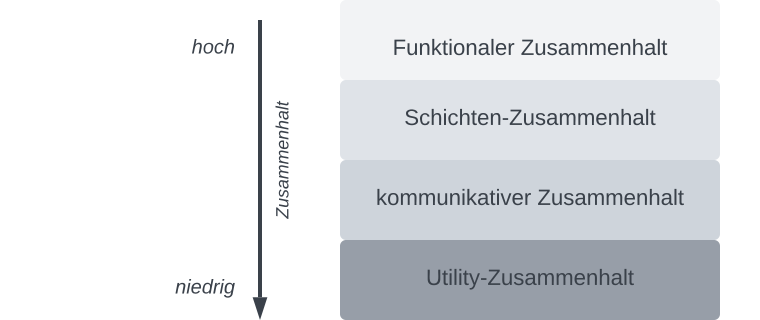
\includegraphics[scale=0.4]{part two/Objektorientierter Entwurf/img/zusammenhalt}
    \caption{Typen des Zusammenhaltes. Der funktionale Zusammenhalt ist verständlicherweise sehr hoch, während der Utility-Zusammenhalt eher schwach ist (Quelle: eigene)}
    \label{fig:zusammenhalt}
\end{figure}


\begin{figure}
    \centering
    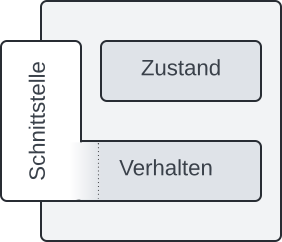
\includegraphics[scale=0.4]{part two/Objektorientierter Entwurf/img/adt}
    \caption{Schematische Darstellung eines abstrakten Datentyps. Verhalten und Zustand kann sowohl intern als auch extern änderbar sein.  (Quelle: eigene)}
    \label{fig:adt}
\end{figure}

\subsection{Lose Kopplung}
\textbf{Kopplungen} sind unvermeidlich, da bestimmte Teile zusammenarbeiten müssen.\\
Dennoch müssen Kopplungen möglichst schwach sein, da die Teile der Software unabhängig voneinander sein sollen.

\subsubsection*{Typen von Kopplungen}
Im Software Engineering wird die Kopplung von Teilen nach Typen klassifiziert, wobei die Stärke der Kopplung unterschiedlich bewertet wird\footnote{
\cite[33 ff.]{Mye75}
} (s. Abbildung~\ref{fig:kopplung}).

\noindent
Mit absteigender Reihenfolge nimmt auch die Stärke der Kopplung in folgender Liste ab:


\begin{itemize}
    \item \textbf{Content-Kopplung}
    \begin{itemize}
    \item ein Teil ändert interne Daten eines anderen Teils
    \item die ändernde Klasse ist von der Struktur der zu ändernden Klasse \textbf{abhängig}
    \item diese Art der Kopplung sollte vermieden werden, bspw. über Zugriffsmodifizierer und Zugriffsmethoden
    \item unerwünschte Seiteneffekte können bspw. über das \textit{Immutable}-Pattern\footnote{
    s. Abschnitt~\ref{subsec:immutable}
    } erreicht werden
    \end{itemize}
    \item \textbf{Common-Kopplung}
    \begin{itemize}
    \item bezeichnet Kopplung über die gemeinsame Verwendung globaler Variablen\footnote{
        bspw. unsachgemäße Verwendung von \textit{static} in Java
    }
    \item führt zu unlesbarem und schwer änderbaren Code, und sollte vermieden werden
    \end{itemize}
    \item \textbf{Stamp-Kopplung}
    \begin{itemize}
    \item ein Objekt wird als Argument einer Methode verwendet
    \item wird der öffentliche Teil der Klasse des Objektes geändert, muss auch die aufrufende Methode geändert werden
    \item zur Vermeidung dieser Kopplung können einfache Variablen übergeben werden\footnote{
        was dann wiederum die \textbf{Data-Kopplung} erhöht, s.u.
    }, oder es werden \textit{Interfaces} oder Klasse genutzt, die weit oben in der Ableitungshierarchie stehen
    \item muss man sich für eine Alternative entscheiden, sollte man bedenken, dass die Anzahl der einfachen Variablen nicht zu groß sein darf
    \end{itemize}
    \item \textbf{Data-Kopplung}
    \begin{itemize}
    \item je mehr Argumente eine Methode hat, desto größer ist die Kopplung mit der benutzenden Komponente\footnote{
    ``The ideal number of arguments for a function is zero (niladic).`` (\cite[40]{Mar08}). Monadische Funktionen sind Funktionen mit einem Argument, dyadische mit zwei, triadische entsprechend mit 3 Argumenten. Polyadische Funktionen sollten laut \textit{Martin} vermieden werden (ebenda).
    }
    \item \textbf{Stamp-Kopplung} und \textbf{Data-Kopplung} bedingen sich gegenseitig: Wird Stamp-Kopplung vermieden, erhöht sich i.d.R. Data-Kopplung, und umgekehrt
    \end{itemize}
    \item \textbf{Routine Call-Kopplung}
    \begin{itemize}
    \item eine Methode ruft eine andere Methode auf
    \item werden sehr viele Methode eines anderen Teils aufgerufen, sollte man die Zerlegung überlegen\footnote{
    s. hierzu auch \textbf{Feature Envy}, ein \textit{Code Smell}, der wie folgt zusammengefasst werden kann: ``a method seems more interested in a class than the one it actually is in`` \cite[80 f.]{Fow99}
    }
    \item werden Methoden immer in gleicher Sequenz aufgerufen, könnte man überlegen, die Sequenz auch als eigenständige Methode zusammenfassen
    \end{itemize}
\end{itemize}

\begin{figure}
    \centering
    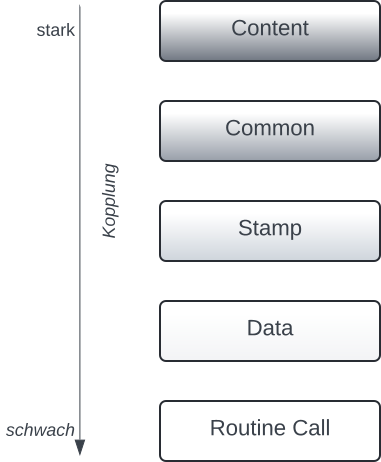
\includegraphics[scale=0.4]{part two/Objektorientierter Entwurf/img/kopplung}
    \caption{Typen von Kopplung, mit absteigender Anordnung wird auch die tatsächliche Kopplung schwächer.  (Quelle: in Anlehnung an \cite[73, Abb. 3.18]{Wed09b})}
    \label{fig:kopplung}
\end{figure}

\subsection{Grundlegende Prinzipien, die weiterhelfen}

\subsubsection*{Abstraktion}
Eine der grundlegenden Prinzipien ist das Prinzip der \textbf{Abstraktion}\footnote{
\textit{Wedemann} merkt an, dass die Bedeutung der Abstraktion für das Software Engineering ``von \textit{Barbara Liskov} und \textit{John Guttag} entdeckt wurde`` (\cite[75, Hervorhebung eigene]{Wed09b}) und erwähnt ein ``sehr anspruchsvolles Buch`` der beiden zu dem Thema, leider ohne weitere Quellenangabe. Man darf vermuten, dass hiermit \cite{LG00} gemeint ist
}.

\noindent
Das Prinzip besagt, dass Bauteile und Abläufe nach außen hin abstrakt sein sollen, also Details weggelassen werden sollten.

\vspace{2mm}
\begin{tcolorbox}[title=Abstraktion]
    \blockquote[{\cite[75, Hervorhebung eigene]{Wed09b}}]{
        Unter \textbf{Abstraktion} versteht man das Herausheben von Wesentlichem, Charakteristischem oder Gesetzmäßigem. Das Prinzip der Abstraktion beruht auf der Beobachtung, dass ein Teil leichter zu verstehen ist, wenn nicht alle Details verstanden werden müssen, sondern nur das Wesentliche.
    }
\end{tcolorbox}
\vspace{2mm}

\subsubsection*{Beispiele für Abstraktion}
\begin{itemize}
    \item Vertikale Schichten sind eine schrittweise Abstraktion von der Hardware
    \item öffentliche Schnittstellen einer Klasse\footnote{
        was als Geheimnisprinzip verstanden werden kann, das \textbf{Content-Kopplung} verhindert
    } können als Abstraktion der Klasse gesehen werden
    \item werden Interfaces zur Vermeidung von \textbf{Stamp-Kopplung} verwendet, ist das Interface die Abstraktion der tatsächlichen Klasse
    \item ein \textbf{Iterator} ist eine Abstraktion des Zugriffs auf eine Datenstruktur
    \item die Ergebnisse von \textbf{Anforderungen}, \textbf{Analyse} und \textbf{Entwurf} können als Abstraktion des zu erstellenden Systems betrachtet werden
\end{itemize}


\subsubsection*{The Law of Demeter}
\textit{Lieberherr}, \textit{Holland}, und \textit{Riel} formulieren 1988 in \cite{LHR88} das \textbf{Law of Demeter}, das das Ziel hat, eine Software möglichst modular zu erstellen.
Dabei ist das Prinzip recht einfach gehalten:

\blockquote[{\cite[325]{LHR88}}]{
    Any method written to obey this Law will only know about the immediate structure of the class to which it is attached.
}

\noindent
\textit{Martin} schreibt hierzu:

\blockquote[{\cite[97 f.]{Mar08}}]{
[...] the law of Demeter says that a method $f$ of a class $C$ should only call the methods of these:
\begin{itemize}
    \item $C$
    \item An object created by $f$
    \item An object passed as an argument to $f$
    \item An object held in an instance variable of $C$
\end{itemize}
}
\noindent
und fasst ebenda das Prinzip folgendermaßen zusammen: ``talk to friends, not to strangers.``\footnote{
s. hierzu auch \url{https://www2.ccs.neu.edu/research/demeter/demeter-method/LawOfDemeter/general-formulation.html}, abgerufen 20.04.2024
}

\subsubsection*{Vermeidung zirkulärer Abhängigkeiten}
Eine \textbf{zirkuläre Abhängigkeit} liegt vor, wenn Beziehungen zwischen Klassen kreisförmig sind (s. Abbildung~\ref{fig:zirkulaer} a).\\
Dadurch können Klassen nicht einzeln entwickelt bzw. getestet werden, was eine sehr starke Kopplung ausdrückt.\\
Eine zyklische Abhängigkeit ist oft ein Fehler im Entwurf.\\
Beruht die Abhängigkeit nicht auf einem Fehler, kann sie durch den Einsatz eines Interfaces aufgelöst werden (s. Abbildung~\ref{fig:zirkulaer} b).).

\begin{figure}
    \centering
    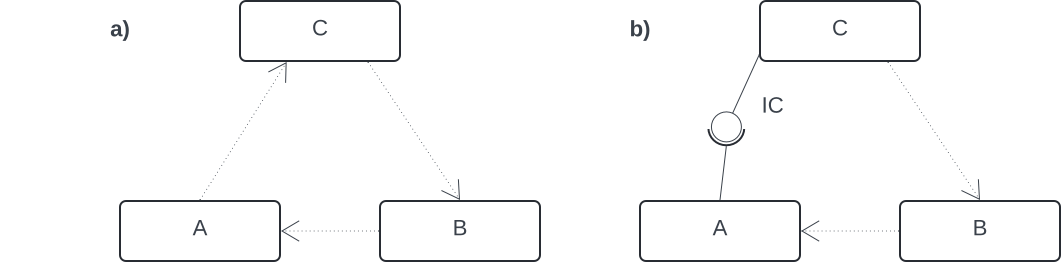
\includegraphics[scale=0.4]{part two/Objektorientierter Entwurf/img/zirkulaer}
    \caption{
        Beispiel für eine zirkuläre Abhängigkeit (a) und deren Auflösung (b).
        (Quelle: in Anlehnung an \cite[76, Abb. 3.19]{Wed09b})
    }
    \label{fig:zirkulaer}
\end{figure}

\subsubsection*{Liskovsches Substitutionsprinzip}
Das \textbf{Ersetzbarkeitsprinzip} wurde bereits im Zusammenhang mit \textbf{Polymorphie} im Abschnitt~\ref{sec:beziehungen-von-klassen} eingeführt.
\section{Verbesserung des Entwurfs durch Refactoring}
Nur selten kann ein neues System von Anfang an so entworfen werden, dass der Entwurf für das gesamte System  durchgängig geeignet und zweckmäßig ist.
Wie in Abschnitt~\ref{sec:vorgehen-beim-entwerfen} diskutiert ist es i.d.R. notwendig, \textbf{iterativ} vorzugehen.
Der Entwurf wird so immer wieder angepaßt.\\
Somit können Schwächen früherer Entwürfe entdeckt und entfernt werden.\\
Sollten sich ansonsten kleine und große Fehler im Entwurf anhäufen, können die dadurch entstehenden starken Kopplungen den Code wenig erweiter- und wartbar machen.\\

\noindent
Es ist allerdings nicht einfach, bereits kleine Mengen existierenden Codes zu ändern.\\
Den Entwurf bestehender Software zu verbessern, ohne dabei die Funktionalität zu ändern, beschreibt \textit{Fowler} in \cite{Fow99}.

\subsubsection*{Vorgehen}
Refactoring besteht aus mehreren Schritten:

\begin{enumerate}
    \item Problematische Stellen identifizieren (sog. \textit{Code Smells})
    \item Refactorings anwenden, um die problematischen Stellen zu verbessern (\textit{Martin}: ``\textit{Heuristics}`` (vgl.~\cite[285 ff.]{Mar08}))
    \item Tests ausführen, um sicherzustellen, dass das Refactoring nicht die Funktionalität geändert hat
\end{enumerate}

\subsubsection*{Refactoring verursacht Aufwand}
Mit Refactoring kann man die Qualität von Code verbessern.
Allerdings zeigt die Praxis, dass fast jeder code kleinere oder größere Probleme hat, die immer weiter verbessert werden können.
Teilweise sind Refactorings mit hohem Aufwand verbunden, wobei nur Qualität, aber nicht Funktionalität verbessert wird.\\
Es sollte deshalb stehts zwischen Dringlichkeit, Aufwand und Auswirkungen abgewogen werden.
\section{Zusammenfassung}

\begin{itemize}
    \item Anforderungen lassen sich bei Projekten vorab nicht genügend festlegen.
    \item Fehlt im Team die Erfahrung oder werden neue Technologien eingesetzt, ist ein ausgereifter Entwurf nicht machbar.
    \item Bei großen Projekten würde man unter diesen Voraussetzungen mit dem Wasserfallmodell nicht flexibel genug sein,
    um auf Änderungen reagieren zu können.
    \item Aus diesem Grund gibt es alternative Modelle, die eingesetzt werden können:
        \begin{itemize}
            \item \textbf{inkrementell}: Aufteilung der Anforderungen, so dass Teilsysteme umgesetzt und an den Kunden ausgeliefert werden können
            Die Teilsysteme werden sequentiell bearbeitet.
            \item \textbf{iterativ}: In Iterationen wird das Projekt in Zeitabschnitte unterteilt, in denen die Anforderungen umgesetzt werden; entsprechend dem Spiralmodell zunächst die risikoreichsten.
            Vorhergehende Ergebnisse werden in darauffolgenden Iterationen weiterbearbeitet.
            Ein bekanntes iteratives Modell ist \textit{RUP}, bei dem einzelne Phasen Ergebnis-Artefakte liefern, wie Anwendungsfälle oder Klassendiagramme.
            \item \textbf{nebenläufig}: Die Aufgaben werden aufgeteilt in parallel (oder nacheinander) bearbeitbare Aufgaben, die dann von den Mitarbeitern umgesetzt werden.
        \end{itemize}
    \item Die genannten Modelle werden häufig nicht isoliert betrachtet, sondern je nach Projekt auch kombiniert, insb. bei dem \textbf{agilen Vorgehen}.
\end{itemize}
\newpage


